\documentclass[conference]{IEEEtran}
\IEEEoverridecommandlockouts
% The preceding line is only needed to identify funding in the first footnote. If that is unneeded, please comment it out.
\usepackage{cite}
\usepackage{amsmath,amssymb,amsfonts}
\usepackage{algorithmic}
\usepackage{graphicx}
\usepackage{textcomp}
\usepackage[brazilian]{babel}
\usepackage{xcolor}
\def\BibTeX{{\rm B\kern-.05em{\sc i\kern-.025em b}\kern-.08em
    T\kern-.1667em\lower.7ex\hbox{E}\kern-.125emX}}
\begin{document}

\title{Extração de informações da Plataforma Lattes}

\author{\IEEEauthorblockN{Alleff Dymytry Pereira de Deus}
\IEEEauthorblockA{\textit{UERGS} \\
Porto Alegre, Brasil \\
alleffdymytry@gmail.com}
}

\maketitle

\begin{abstract}
Este documento reune as informações necessárias para o entendimento da aplicação desenvolvida bem como as formas de modificação da mesma para obter outras informações. Dentro deste documento serão apresentadas as funções realizadas bem como as adversidades enfrentadas e os meios de contornar estas adversidades.
\end{abstract}

%\begin{IEEEkeywords}
%component, formatting, style, styling, insert
%\end{IEEEkeywords}

\section{Introdução}
As informações da vida acadêmica de cada professor possui um grande apreço para o desenvolvimento e propagação no incentivo a educação, estas informações normalmente contidas na plataforma Lattes. Todavia estas informações acabam sendo centralizadas e não possuindo uma separação em relação a cada instituição, sendo assim a extração das informações se faz necessária para a utilização destas informações em outras plataformas. As informações extraídas podem ser utilizadas em novas plataformas, podendo ser utilizadas e disponibilizadas em formas diferentes, alguns exemplos: tamanho diferente, filtros por áreas, classes de texto, etc.

O objetivo do presente trabalho é o desenvolvimento de uma aplicação para a extração das informações dos professores da Universidade Estadual do Rio Grande do Sul para a sua utilização em uma plataforma própria da universidade. As informações extraídas são armazenadas em arquivos para uso futuro na plataforma.

\section{Fundamentação Teórica}

Para o desenvolvimento da aplicação proposta os seguintes conhecimentos e ferramentas foram necessários.

\subsection{Python}

A linguagem de programação Python foi utilizada para o desenvolvimento da aplicação devido as seguintes vantagens: alto desempenho, orientada a objetos, grande acervo de bibliotecas e integração com as mais diversas plataformas.

\subsection{HTML}
A linguagem de programação de páginas web HTML (HyperText Markup Language - Linguagem de Marcação de Hipertexto) é padrão na representação das mais diversas páginas na internet. A estrutura do HTML é dividida em blocos, sempre possuindo um bloco inicial e um bloco final, estes blocos represemtam os elementos que são possíveis de serem incluídos na páginas.

\subsection{Selenium}
O Selenium é um conjunto de bibliotecas e ferramentas que permitem a automação em navegadores web. É possível emular ações programadas dentro dos navegadores, assim é possível testar funções desenvolvidas e analisar possíveis falahas. O selenium possui biblioteca para o seu uso com a linguagem python, 


\section{Materiais e Métodos}\label{AA}
As etapas da aplicação foram desenvolvidas utilizando a linguagem Python em conjunto com a biblioteca Selenium. A aplicação foi desenvolvida e testada em uma máquina com um processador AMD Ryzen 5 3400G de 3,7GHz, memória RAM de 16GB e placa de vídeo Radeon RX 590 de 8GB de VRAM.

O fluxo de funcionamento da aplicação proposta pode ser notada na Figura \ref{fluxo}, onde para cada professor é realizado o fluxo do início ao fim.

\begin{figure}[htbp]
\centerline{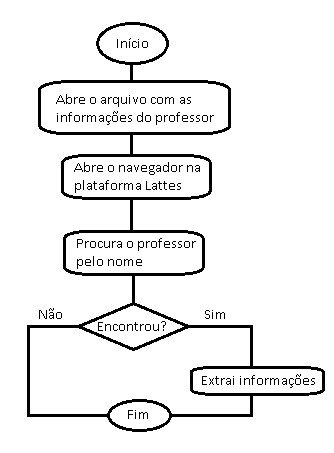
\includegraphics[width=0.3\textwidth]{fluxo.png}}
\caption{Fluxograma da aplicação.}
\label{fluxo}
\end{figure}

\subsection{Abrir Arquivos}
A etapa de abertura dos arquivos se refere ao processo de abrir um arquivo previamente disposto para a aplicação contendo o nome completo de cada professor. O arquivo que contêm o nome de cada professor deve ser salvo no formato de \textit{.csv} e cada nome deve estar em uma nova linha, um exemplo de como as informações deve ser organizadas esta disposta na Figura \ref{info}.

\begin{figure}[htbp]
\centerline{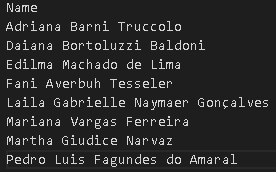
\includegraphics[width=0.3\textwidth]{info.png}}
\caption{Exemplo do arquivo de informações do professor.}
\label{info}
\end{figure}

A primeira linha do arquivo deve conter a informação de cada coluna do arquino, neste caso o nome do professor, caso mais informações sejam adicionadas deve-se separar cada informação por virgulas e colocar uma descrição do que foi adicionado, como por exemplo se a data de nascimento for adicionada, a primeira linha da Figura \ref{info} seria: "Name,dataNasc".

\subsection{Abrir o Navegador}

A biblioteca Selenium possui funções para a abertura automática do navegador web escolhido na aplicação, neste caso o navegador Chromium foi o utilizado, contudo para tal abertura é necessário baixar o arquivo de driver do Selenium para o navegador escolhido. O arquivo deve ser colocado na mesma pasta que a aplicação.

O navegador tem sua página diretamente direcionada para a página de pesquisa de pesquisadores da plataforma Lattes, facilitando a busca dos professores. Com a janela do navegador na página correta, foi necessário realizar uma análise no código fonte da página em questão para obter o valor da caixa de inserção de texto, assim sendo possível colocar o nome do professor na pesquisa. Com o valor HTML do elemento, foi necessário realizar a busca utilizando a função de pesquisa de elemntos do Selenium, esta pesquisa pode ser feita com diversos valores, como por exemplo: o identificador do elemento, a classe, o caminho xpath e entre outros. A forma como a análise foi realizada pode ser vista na Figura \ref{html}.

\begin{figure}[htbp]
\centerline{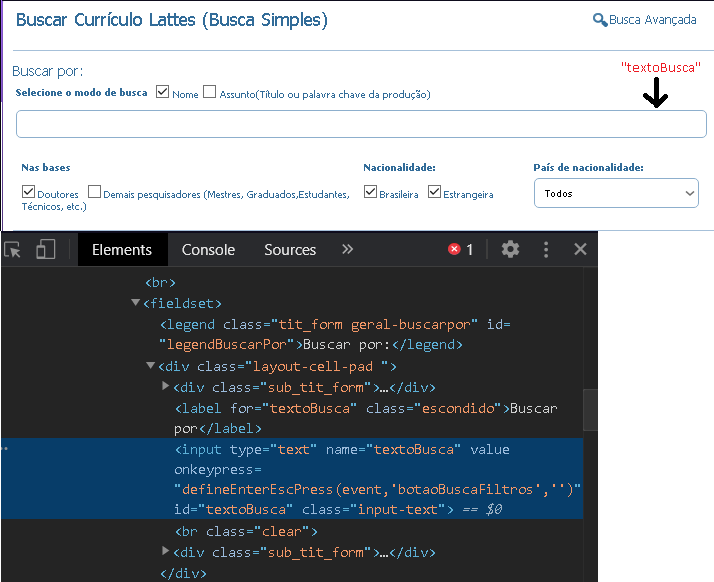
\includegraphics[width=0.4\textwidth]{html.png}}
\caption{Análise do código HTML.}
\label{html}
\end{figure}

A extração das informações contidas em uma página web ocorre de forma manual, sendo necessário analisar previamente as informações que devem ser extraídas.

\subsection{Pesquisa Professor}
O elemento de inserção de texto deve ser encontrado na página web previamente, assim que o elemento é localizado é realizado a inserção do nome completo do professor e a inserção da tecla "ENTER" é realizada em seguida, esta inserção da tecla "ENTER" realiza a pesquisa, assim não é necessário realizar a procura do botão de pesquisa na página.

A pesquisa é realizada e a página é recarregada com as informações do site, as informações disponibilizadas são os perfis dos professores na base do Lattes. Estes perfis são clicáveis, abrindo uma janela para o redirecionamento para o currículo da pessoa em questão. O currículo aberto gera uma nova página no navegador, sendo assim é necessário fazer a troca de página para poder obter as informações do professor. Caso a pessoa não seja encontrada dentro de um tempo limite, a aplicação avisa que a pessoa em questão não foi encontrada e começa a pesquisar o próximo.

A troca de páginas segue o seguinte fluxo de operação: 1) deve-se obter todas as páginas abertas em uma lista, 2) salvar em uma variável o valor da página atual, para realizar o retorno posteriormente, 3) selecionar a página que não tem o valor da página original, 4) realizar a troca de página. A troca é realizada automaticamente pelas funções do Selenium. Com a página trocada é possível obter as informações da pessoa.

As informações extraídas da página são tratadas, para não conter espaços em branco e informações desnecessárias ou dispensáveis no atual momento. As informações tratadas são armazenadas em um arquivo no formato \textit{.json}, o arquivo possui o nome da pessoa encontrada. Um exemplo do tratamento e organização das informações extraídas pode ser notada na Figura \ref{json}.

\begin{figure}[htbp]
\centerline{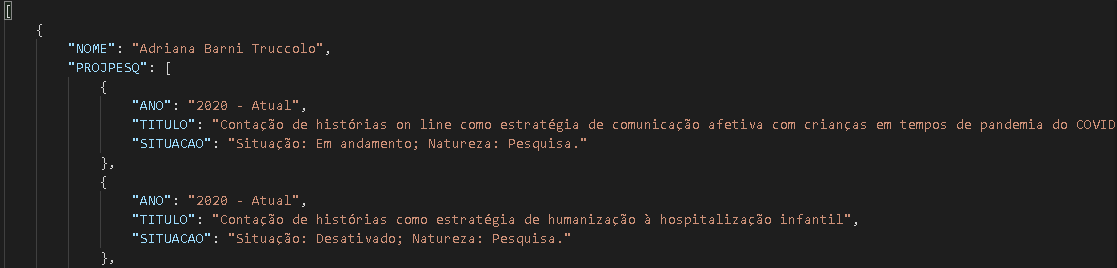
\includegraphics[width=0.5\textwidth]{json.png}}
\caption{Exemplo das informações extraídas.}
\label{json}
\end{figure}

As informações armazenadas em um arquivo no formato \textit{.json} pode ser utilizada em diferentes aplicações, além de possuir um formato de descrição leve, onde caso necessário que uma nova informação seja adicionada manualmente, não seja um tarefa árdua, já que o padrão de inserção de informações pode ser copiado das informações anteriores.
\section{Resultados e Discussões}

Com o desenvolvimento da aplicação proposta, foi possível obter as informações de projetos de pesquisa e projetos de extensão de cada professor da Universidade Estadual do Rio Grande do Sul. Contudo algumas dificultades foram enfrentadas, sendo estas dificuldades discutidas nesta seção.

\subsection{Desrcrição dos Projetos}
As informações descritas nos perfis de cada professor possuem algumas informações em comum, como por exemplo: 1) ano do projeto, 2) nome do projeto e 3) situação do projeto. Contudo a descrição é uma informação que nem todos os projetos possuem, fazendo com que não se possa utilizar uma única técnica de extração e tratamento das informações, um exemplo desta situação pode ser vista na Figura \ref{prob1}. Para contornar esta adversidade foi necessário realizar uma análise nas informações extraídas, onde mesmo que um projeto não contivesse uma descrição, o título de \textit{"Descrição:"} seria inserido junto de cada projeto extraído. A solução para contorno da falta de descrição nos projetos, faz com que seja possível utilizar um padrão de extração para todos os projetos de cada professor.

\begin{figure}[htbp]
\centerline{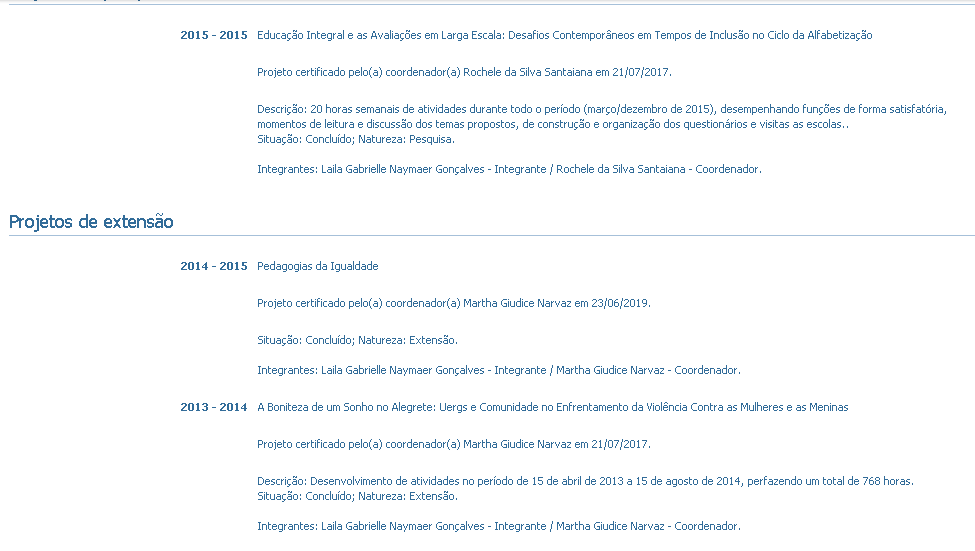
\includegraphics[width=0.5\textwidth]{exemplo1.png}}
\caption{Exemplo das informações extraídas.}
\label{prob1}
\end{figure}

\subsection{Nomes Repetidos}
As pessoa cadastradas na plataforma Lattes podem possuir nomes parecidos ou até mesmo iguais, com isso existe a possibilidade de acesso de um perfil que não pertence ao professor correto, ver Figura \ref{mnome}. Esta situação pode se apresentar de duas excessões diferentes, sendo elas: 1) existe pessoas com partes do nome iguais, contudo o nome completo pode distinguir quem é o correto e 2) quando o nome completo é igual a de outra pessoa ou pessoas.

\begin{figure}[htbp]
\centerline{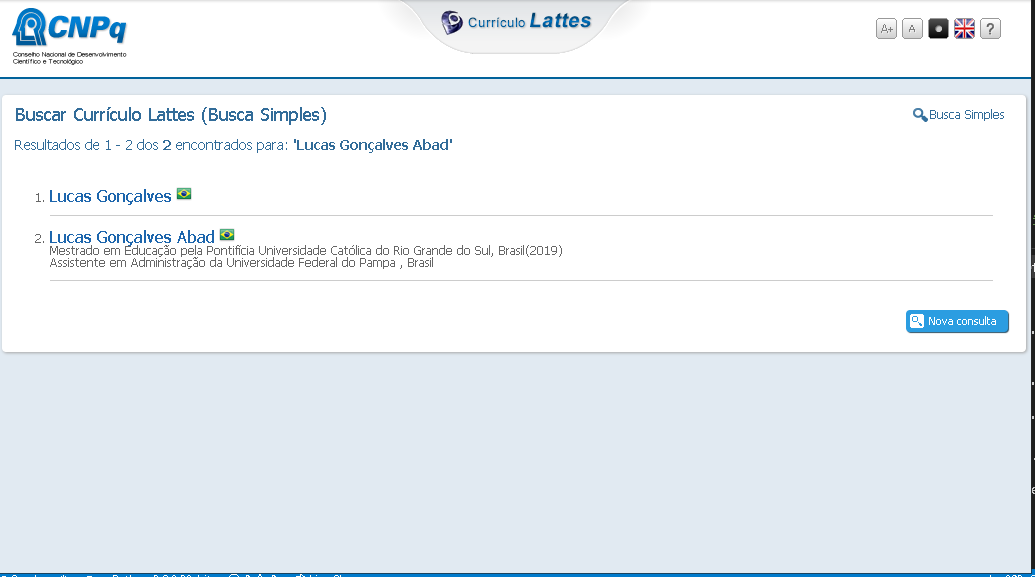
\includegraphics[width=0.5\textwidth]{exemplo2.png}}
\caption{Exemplo de perfis com nomes iguais.}
\label{mnome}
\end{figure}

A primeira excessão foi solucionada realizando a pesquisa do elemento que possuía o nome completo inserido no campo de pesquisa , onde o currículo somente era aberto se o nome estivesse exatamente igual. Já a segunda excessão não possui uma solução, devido as múltiplas possibilidades, assim se faz necessário a utilização de outra informação do que o nome, poderia se utilizar o identificador único do perfil do professor.

A solução para a segunda excessão necessita de um pré-processamento no arquivo de informações dos professores, onde seria necessário os identificadores de todos os perfis de cada professor na plataforma Lattes, assim caso o professor não fosse encontrado pelo seu nome, seria procurado pelo seu identificador único.

\subsection{Nome Incorreto}
As informações dos professores são carregadas do arquivo que foi processado previamente, com isso é necessário que todas as informações que estão neste arquivo estejam corretas. Todavia existe a possibilidade de que o nome armazenado no arquivo não esteja correto ou não seja o nome cadastrado na plataforma Lattes. Sendo assim é necessário o tratamento do arquivo previamente. Caso o nome esteja correto mas o seu perfil não seja encontrado, foi necessário deixar de pesquisar o perfil do professor em questão, já que não há uma forma de comprovar se o nome está correto ou se o nome do arquivo e o nome do perfil na plataforma são os mesmos, um exemplo deste problema pode ser visto na Figura \ref{notfound}.

\begin{figure}[htbp]
\centerline{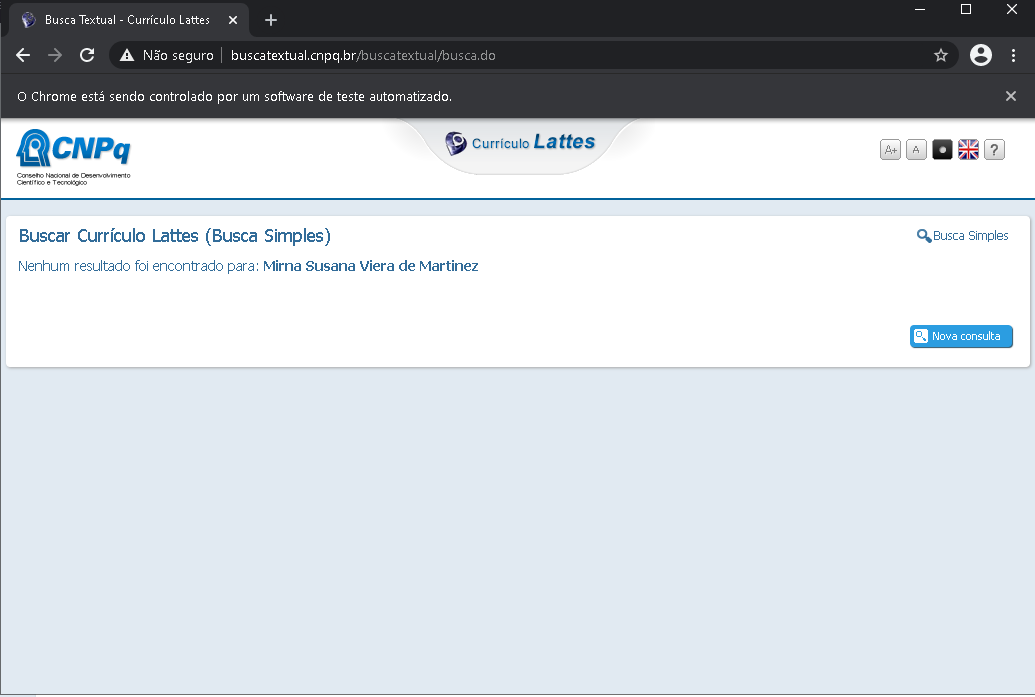
\includegraphics[width=0.5\textwidth]{exemplo4.png}}
\caption{Exemplo de nome incorreto.}
\label{notfound}
\end{figure}

\subsection{Pesquisa não carregada}

As pesquisas realizadas em sua grande maioria sempre retornava uma página com os perfis encontrados ou uma página sem perfis. Contudo durante os testes ocorreram erros no carregamento dos perfis, onde a busca de um professor retornava positiva porém o seu perfil não estava acessível para a aplicação, um exemplo deste erro pode ser notado na Figura \ref{noperfil}.

\begin{figure}[htbp]
\centerline{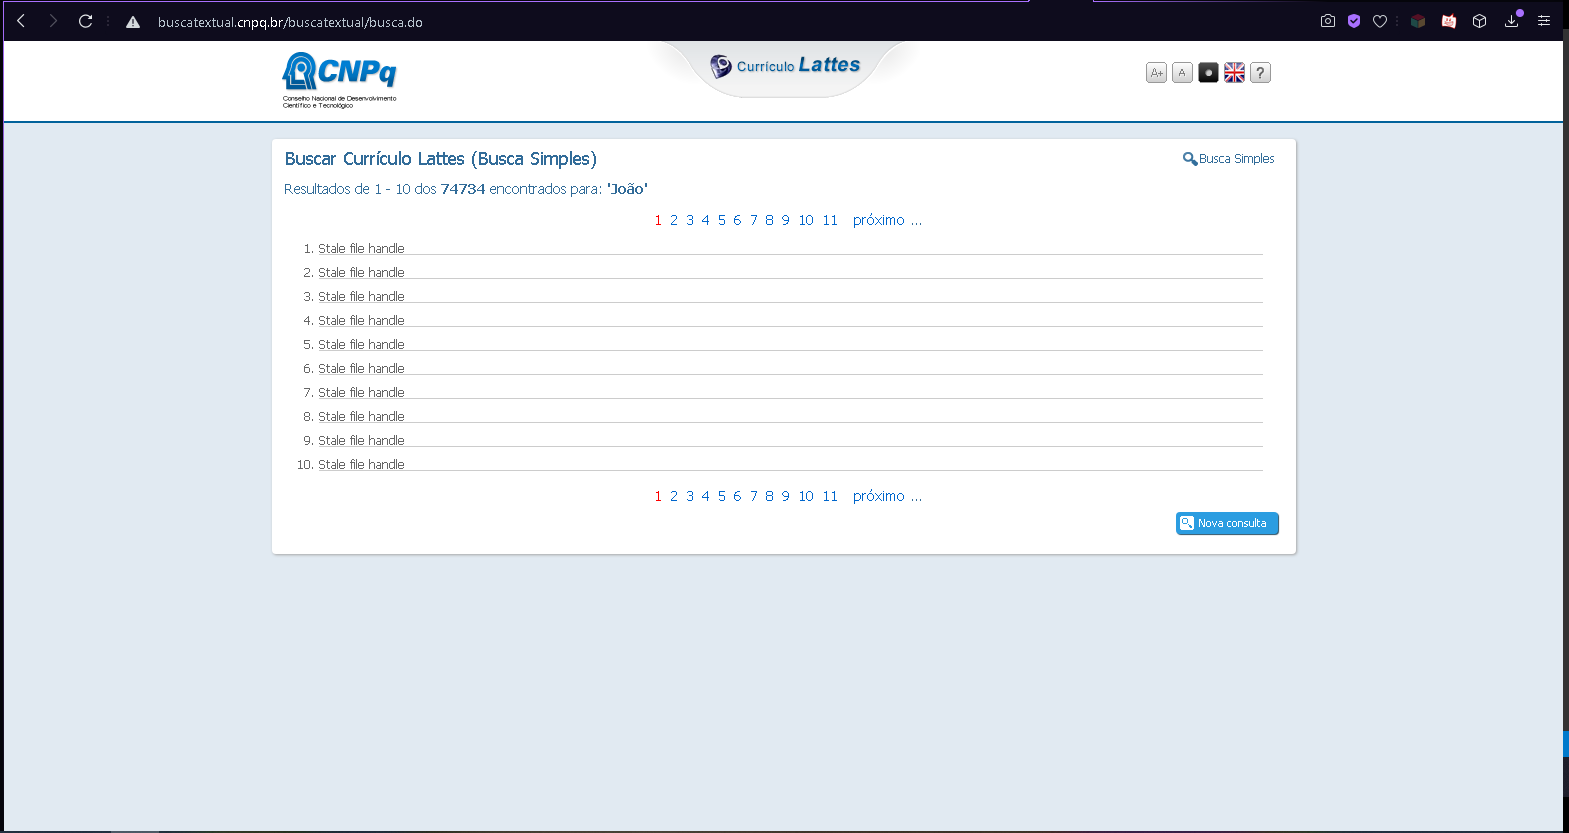
\includegraphics[width=0.5\textwidth]{exemplo3.png}}
\caption{Exemplo de nome incorreto.}
\label{noperfil}
\end{figure}

O erro dos perfis não serem disponibilizados não foram resolvidos devido a possibilidade de um mal carregamento das informações da plataforma, sendo necessário um melhor estudo na ocorrência deste erro, para assim estipular uma forma de contornar este erro. Uma possibilidade seria a de caso este erro ocorra, realizar a pesquisa do professor novamente.

\section{Conclusão}
As informações extraídas da plataforma Lattes devem ser tratadas, pois podem possuir espaços e informações desnecessárias devido a construção da página web.

A aplicação desenvolvida pode ser utilizada para obter as informações de um conjunto de professores, mesmo que seja necessário somente a informação de um professor, se estiver dentro de um arquivo seguindo o padrão apresentado neste trabalho, não haverá problemas.

A aplicação desenvolvida não pode ser utilizada para a extração de qualquer informação do perfil de um professor, já que ele foi pensado até o presente momento para somente extraír as informações de projetos de pesquisa e extensão de forma automática. Para a extração de novas informações é necessária a refatoração do código fonte da aplicação para que seja extraída a informação desejada.

\section*{Apêndice}
Os códigos da aplicação podem ser encontrados na plataforma de versionamento de arquivos Github no link https://github.com/DarkDym/GDL.

\begin{thebibliography}{00}
\bibitem{b1} Selenium, https://www.selenium.dev/documentation/en/.
\bibitem{b2} Python, https://www.python.org .
\bibitem{b3} HTML, https://pt.wikipedia.org/wiki/HTML .
\bibitem{b4} Plataforma Lattes, http://buscatextual.cnpq.br/buscatextual/busca.do .
\end{thebibliography}

\end{document}
